\documentclass[ngerman,12pt,numbers=noenddot]{scrreprt}
\KOMAoptions{paper=a4}
\KOMAoptions{twoside=false}
%\KOMAoptions{footinclude=false}
%\KOMAoptions{headinclude=false}

%\usepackage[ascii]{inputenc}
%\usepackage[T1]{fontenc}
%\usepackage[ngerman,english]{babel}
\usepackage[latin1]{inputenc}
\usepackage{ngerman}
\usepackage{enumerate}
%\usepackage{eurosym}
\usepackage{color}

\usepackage{hyperref}
%\hypersetup{
%	pdftex, 
%	colorlinks=true, 
%	linkcolor=blue, 
%	citecolor=blue, 
%	filecolor=blue, 
%	urlcolor=blue, 
%	pdftitle=Ipponboard Handbuch, 
%	pdfauthor=Florian M\"ucke, 
%	pdfsubject=, 
%	pdfkeywords=
%}
%\usepackage[pdftex]{graphicx}
\usepackage{graphicx}

\usepackage[T1]{fontenc}
\usepackage{avant}
\renewcommand*\familydefault{\sfdefault} 

\usepackage{fontspec} 
%\defaultfontfeatures{Mapping=tex-text} 
%\setmainfont{URW Gothic L} %PT Sans


\newcommand*{\ipponboard}{
\fontspec[
  %FakeBold=1.2
]{Cuprum}
\selectfont 
\textsc{Ipponboard}}

\newcommand*{\mybox}[1]{\vskip 0.5em 
	\fbox{\parbox{\textwidth}{#1}}
	\vskip 0.5em
}




% Outline numbering
%\setcounter{secnumdepth}{4}
%\renewcommand\thesection{\arabic{section}}
%\renewcommand\thesubsection{\arabic{section}.\arabic{subsection}}
%\renewcommand\thesubsubsection{\arabic{section}.\arabic{subsection}.\arabic{subsubsection}}
%\renewcommand\theparagraph{\arabic{section}.\arabic{subsection}.\arabic{subsubsection}.\arabic{paragraph}}

% Page layout (geometry)
%\setlength\voffset{-1in}
%\setlength\hoffset{-1in}
%\setlength\topmargin{1.499cm}
%\setlength\oddsidemargin{1.499cm}
%\setlength\textheight{15.009cm}
%\setlength\textwidth{26.702cm}
%\setlength\footskip{1.497cm}
%\setlength\headheight{0.998cm}
%\setlength\headsep{0.499cm}

% Footnote rule
\setlength{\skip\footins}{0.119cm}
\renewcommand\footnoterule{\vspace*{-0.018cm}\setlength\leftskip{0pt}\setlength\rightskip{0pt plus 1fil}\noindent\textcolor{black}{\rule{0.25\columnwidth}{0.018cm}}\vspace*{0.101cm}}

% Pages styles
\makeatletter
\newcommand\ps@Standard{
  \renewcommand\@oddhead{{\ipponboard} 0.4.1}
  \renewcommand\@evenhead{\@oddhead}
  \renewcommand\@oddfoot{{\textcopyright} Florian M\"ucke, E-Mail: dev@mueckeimnetz.de, Stand: 13.10.2010\hfill \thepage{}/?}
  \renewcommand\@evenfoot{\@oddfoot}
  \renewcommand\thepage{\arabic{page}}
}
\makeatother
\pagestyle{Standard}

% footnotes configuration
\makeatletter
\renewcommand\thefootnote{\arabic{footnote}}
\makeatother
\title{{\ipponboard} Handbuch}
\subtitle{Version 0.4.2}
%\author{Florian M\"ucke}
\date{\today}


\begin{document}
\maketitle


{\centering\bfseries\itshape
Dieses Dokument wird gerade \"uberarbeitet. Der vorliegende Inhalt kann und wird sich \"andern. Es besteht kein Anspruch auf Vollst\"andigkeit! \par}


{{\ipponboard} \textsf{\textmd{Anzeigesystem}}
{ Version 0.4.1 \par}

\bigskip
\bigskip


{\centering
Copyright \textrm{{\textcopyright}} 2010 Florian M\"ucke
\par}

{\centering
Webseite: \url{http://flo.mueckeimnetz.de/ipponboard}
\par}

{\centering
\ Support, Bugtracking: \url{http://ipponboard.origo.ethz.ch/} 
\par}

\newpage
\section*{Lizenz}

{\ipponboard} Copyright \textrm{{\textcopyright}} 2010 Florian M\"ucke.

Creative Commons Lizenz: Namensnennung-Keine Bearbeitung 3.0 Unported \url{http://creativecommons.org/licenses/by-nd/3.0/deed.de}

Lizenzen f\"ur besondere Dateien sind folgende:
\begin{itemize}
	\item Qt (\texttt{QtCore4.dll}, \texttt{QtGui4.dll}): LGPL
	\item Microsoft Visual C++ CRT (\texttt{msvcm*.dll}, \texttt{msvcp*.dll}, \texttt{msvcr*.dll}): Visual Studio 2008/2010 License
	\item Sounddateien: Public Domain
\end{itemize}

Verwendete Bibliotheken:
\begin{itemize}
	\item Qt framework
	\item Boost C++ libraries (\href{http://www.boost.org/}{www.boost.org})
\end{itemize}
\mybox{\itshape\textbf{Hinweis:} Sie d\"urfen {\ipponboard} frei auf beliebig vielen Rechnern innerhalb des Testzeitraums verwenden und das Programm auch in unver\"anderter Form unentgeltlich an dritte weitergeben.}
Weitere Informationen entnehmen Sie bitte der \texttt{Lizenz.txt}-Datei.




\section*{Danksagung}
Mein besonderer Dank gilt folgenden Leuten:
\begin{itemize}
	\item Heini Sch\"afer -- f\"ur die Idee, den Ansporn, die Kritik und das Know-How
	\item Meiner Frau Anja f\"ur ihre Geduld
	\item Christophe Henry -- f\"ur MSM Bibliothek (jetzt: boost msm)
	\item Nokia/Trolltech -- f\"ur die Qt Bibliothek
	\item ETH Z\"urich -- f\"ur Origo subversion project hosting
\end{itemize}

sowie folgenden Vereinen f\"ur Vertrauen und Feedback:
\begin{itemize}
	\item TSV K\"onigsbrunn
	\item Post SV Telekom Augsburg
	\item TSV Peiting
	\item \dots
\end{itemize}


%\setcounter{tocdepth}{10}
\renewcommand\contentsname{Inhalt}
\tableofcontents


\chapter{Einleitung}
{\ipponboard} ist ein fortschrittliches Anzeigesystem f\"ur die Kampfzeit und die Kampfpunkte, das speziell f\"ur den Judowettkampf entwickelt wurde. Bei der Entwicklung wird auf die folgenden Punkte besonderes Augenmerk gelegt:
\begin{itemize}
	\item ausgezeichnete Lesbarkeit
	\item einfache Bedienung
	\item unkomplizierter Einsatz
\end{itemize}

Das Programm wird prinzipiell von einem PC (Laptop) aus bedient und mit Maus oder Gamepad gesteuert. {\ipponboard} verwaltet zwei Anzeigen, eine externe f\"ur die K\"ampfer/Betreuer/Publikum und eine f\"ur die Zeitnehmer. Die Anzeige der Zeitnehmer ist dabei gespiegelt, damit sie besser zu den K\"ampfern zugeordnet werden kann.

\section{Anzeige}
Die Anzeige besteht im Wesentlichen aus f\"unf Bereichen:
\begin{itemize}
	\item \textit{Kampfzeit:} Diese befindet sich am unteren Rand der Anzeige. Ist der Kampf unterbrochen wird die Kampfzeit \textit{rot} dargestellt, ansonsten \textit{gelb}.
	\item Wertungen: Die Wertungen sind auf der Seite des jeweiligen K\"ampfers gruppiert und in der jeweiligen Farbkombination gehalten (Wei{\ss} auf Blau bzw. Schwarz auf Wei{\ss}). Die Strafen sind durch rote Punkte symbolisiert.
	\item Haltegriffzeit
	\item Kampfinformationen (Mattennummer, aktuelle Gewichtsklasse)
	\item Namen der K\"ampfer
\end{itemize}

\subsection[Prim\"are Anzeige]{Prim\"are Anzeige}
\begin{center}
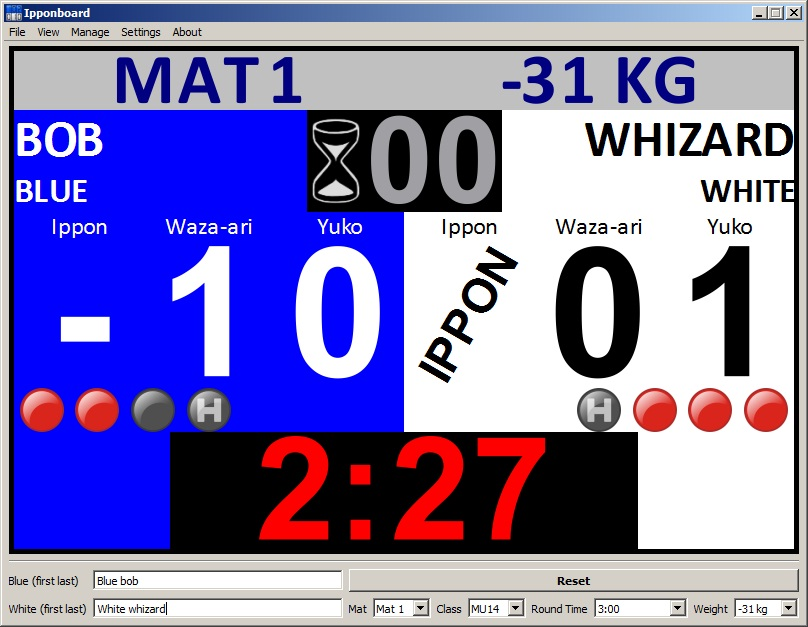
\includegraphics[width=0.8\textwidth]{Anleitung-img001.jpg}
\end{center}
Die prim\"are Anzeige dient als zentrale Steuereinheit. Auf ihr sind alle Informationen verf\"ugbar und einstellbar:
\begin{itemize}
	\item Kampf- und Haltegriffzeit starten/stoppen/(zur\"uck-)setzen
	\item Kampf zur\"ucksetzen
	\item Namen der K\"ampfer \"andern
	\item Wertungen setzen/zur\"ucknehmen
	\item Kampfinformationen (Mattennummer, aktuelle Gewichtsklasse) \"andern
\end{itemize}

\subsection{Sekund\"are (externe) Anzeige}
Im Unterschied zur prim\"aren Anzeige werden auf der sekund\"aren nur die f\"ur das Kampfgeschehen wesentlichen Details angezeigt:

\begin{itemize}
	\item nur die Wertungen bis Waza-ari (Ippon wird blinkend dar\"ubergelegt)
	\item nur die aktiven Strafen
	\item nur die aktive Haltegriffzeit
\end{itemize}

Zudem reagiert die sekund\"are Anzeige nicht auf Eingaben mit der Maus.

\mybox{\itshape\textbf{Tipp:}\\
Aktivieren/Deaktivieren l\"asst sich die sekund\"are Anzeige \"uber den Hotkey \texttt{F2}.}

Ob die zweite Anzeige beim Programmstart gleich angezeigt werden soll,
oder auf welchem Bildschirm diese ausgegeben weird, l\"asst sich in den
\textit{Programmeinstellungen} festlegen.

Wie sie Ihren Rechner f\"ur den Zweischirmbetrieb ({\quotedblbase}Dual-View``) konfigurieren m\"ussen, k\"onnen Sie im Anhang: \textit{Computer f\"ur Zweischirmbetrieb vorbereiten} nachlesen.


\section[Programmeinstellungen]{Programmeinstellungen}

\label{bkm:Programmeinstellungen}
Die Programmeinstellungen finden Sie im Anwendungsmen\"u unter Einstellungen. Sie bieten Ihnen Zugriff auf verschiedene \textit{allgemeine} Optionen zur Anpassung des Programms:

\begin{itemize}
	\item Sekund\"are Anzeige konfigurieren
	\item Farben und Schriftart f\"ur den Info-Bereich \"andern
	\item Farben f\"ur K\"ampfer/Wertungen \"andern
	%\item TODO:Schriftart f\"ur die Kampfzeit \"andern
	\item Sounddatei f\"ur das Signal des Zeitnehmertisches ausw\"ahlen
	%\item TODO: Standardeinstellungen wiederherstellen
\end{itemize}

Neben den allgemeinen Optionen lassen sich im Einstellungsmen\"u auch die Kn\"opfe des Gamepads neu belegen.

\chapter{Steuerung}

{\ipponboard} kann sowohl mit der Maus als auch mit dem Gamepad bedient werden\footnote{Die Steuerung \"uber die Tastatur ist f\"ur sp\"atere Versionen geplant.}. Damit das aktuell Kampfgeschehen m\"oglichst unkompliziert und intuitiv wiedergegeben werden kann, l\"asst sich dieses vollst\"andig mit einem der beiden Eingabeger\"ate
steuern.

Die Steuerung \"uber die Maus mag zun\"achst einfacher erscheinen, da dieses Eingabeger\"at f\"ur die meisten vertraut ist und man die Anzeige intuitiv via Klicks ansprechen kann.

Unsere Erfahrungen haben jedoch gezeigt, dass mit dem Gamepad ein wesentlich entspannteres Bedienen als mit der Maus m\"oglich ist. Daher m\"ochten wir Ihnen die Steuerung mit dem Gamepad mit folgenden Gr\"unden besonders ans Herz legen:

\paragraph*{Vorteile der Gampad-Steuerung}
\begin{enumerate}
	\item Alles im Griff
	\item Volle Konzentration auf das Kampfgeschehen
	\item Entspannt zur\"ucklehnen
	\item Coolness-Faktor
\end{enumerate}

Zu i.: Sie k\"onnen mit einem handels\"ublichen USB-Gamepad auf alle wesentlichen Funktionen per Knopfdruck zugreifen -- egal ob Haltegriffanzeige, Kampfzeit, Wertungen oder Strafen. Dabei ist die linke Hand f\"ur den linken K\"ampfer und die rechte f\"ur den rechten zust\"andig.

Zu ii.: Der Blick muss nicht st\"andig zwischen Anzeigetafel und Matte hin- und herwechseln. Punkte k\"onnen direkt eingegeben werden und es muss nicht st\"andig der Mauszeiger gesucht und erst umst\"andlich auf
das Wertungssymbol geschoben werden. Ein Knopfdruck und ein gelegentlicher fl\"uchtiger Kontrollblick reichen v\"ollig aus.

Zu iii.: Das Beste daran: man kann sich ganz entspannt auf dem Stuhl zur\"ucklehnen, anstatt konzentriert und angespannt vor der Maus zu sitzen.

Zu iv.: F\"ur den Einsatz bei der Jugend sollte man den {\quotedblbase}Coolness-Faktor`` nicht untersch\"atzen -- so bedienen will wirklich jeder!

\section{Aufbau der Steuerung}
\subsection{Maus-Steuerung}
Das Programm kann komplett mit der Maus gesteuert werden. Hierf\"ur muss lediglich auf die jeweiligen Felder in der prim\"aren (eingebetteten) Anzeige oder auf die entsprechenden Kn\"opfe in der Oberfl\"ache geklickt werden.

\paragraph{Punkte vergeben und zur\"ucknehmen}
Um Punkte zu vergeben bzw. diese wieder zur\"uckzunehmen muss lediglich in das jeweilige Feld geklickt werden. Dabei gilt Folgendes:

\begin{itemize}
	\item \textbf{Punkt geben:} linke Maustaste
	\item \textbf{Punkt zur\"ucknehmen:} rechte Maustaste
\end{itemize}

\paragraph{Zeit starten/stoppen (Hajime/Matte)}
Die Kampfzeit kann mit Linksklick gestartet (gelb) und gestoppt (rot)werden.

\paragraph{Haltegriffzeit starten/stoppen (Osaekomi / Toketa)}
{Zum Starten der Haltezeit muss auf das {\quotedblbase}00``-Feld neben der Sanduhr geklickt werden. Der Haltegriff wird hierbei zun\"achst automatisch f\"ur Blau angezeigt. \"Uber das Kontextmen\"u dieses Feldes (Rechtsklick) kann der Haltegriff dann Wei{\ss} zugeordnet werden, falls n\"otig.}

Erneutes Anklicken des Feldes mit links stoppt die Haltegriffzeit.

Die Zeit wird jetzt so lange angezeigt, bis entweder erneut ein Haltegriff ausgel\"ost wird, oder die Hauptzeit nach Anhalten wieder l\"auft (=\textit{Hajime}).

\subsection{Gamepad-Steuerung}
\paragraph{Tasten einstellen}

\dots

\begin{center}
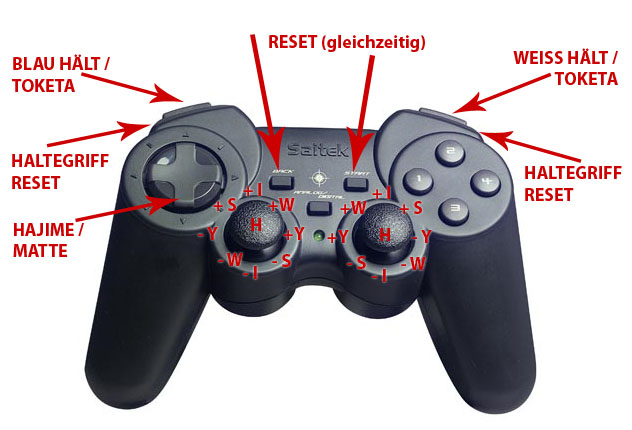
\includegraphics[width=0.8\textwidth]{Anleitung-img002.jpg}
\end{center}
\paragraph[Punkte vergeben und zur\"ucknehmen]{Punkte vergeben und zur\"ucknehmen}
Die Punkte werden \"uber die beiden Analog-Sticks vergeben. Dabei entsprechen beim \textbf{blauen} K\"ampfer folgende Richtungen den jeweiligen Punkten:
\begin{center}
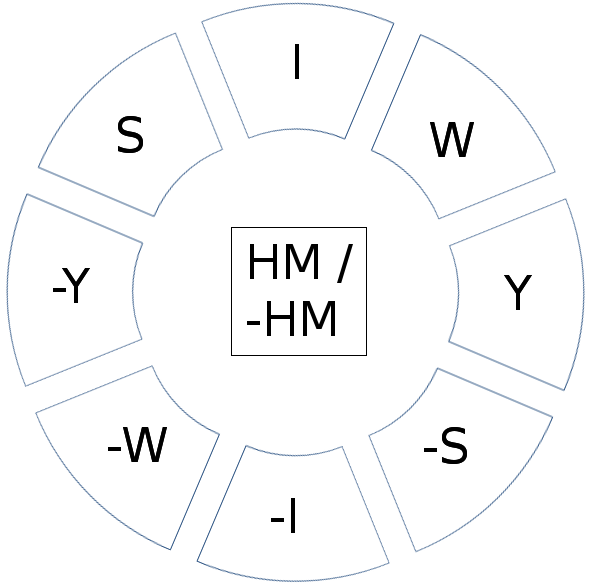
\includegraphics[width=5.211cm,height=5.17cm]{Anleitung-img003.png}
\end{center}
\begin{itemize}
	\item {\bfseries Ippon:} nach oben
	\item {\bfseries Ippon zur\"ucknehmen}: nach unten
	\item {\bfseries Waza-ari:} rechts oben
	\item {\bfseries Waza-ari zur\"ucknehmen:} links unten
	\item {\bfseries Yuko:} rechts
	\item {\bfseries Yuko zur\"ucknehmen:} links
	\item {\bfseries Shido:} links oben
	\item {\bfseries Shido zur\"ucknehmen:} rechts unten
	\item {\bfseries Hansokumake (zur\"ucknehmen):} Analog-Stick dr\"ucken
\end{itemize}

F\"ur den wei{\ss}en K\"ampfer sind die Richtungen einfach spiegelverkehrt.

\textbf{Vorsicht:} Bitte beachten Sie, wie die jeweiligen Achsen des Gamepads konfiguriert sind.Eventuell m\"ussen diese in den Einstellungen invertiert werden.

\mybox{\itshape
{\bfseries Tipp:\newline}
Um herauszufinden, wie das jeweilige Gampad ausgerichtet ist, kann man das mitgelieferte Programm \texttt{GamepadDemo.exe} verwenden. Dort sieht man, wie die jeweiligen Achsen ausgerichtet sind und wie die
Kn\"opfe intern nummeriert sind.}

\paragraph{Zeit starten/stoppen (Hajime/Matte)}
Die Hauptzeit wird mittels der \textit{Nach-Unten}-Taste des Drehkreuzes des Gamepads gestartet oder gestoppt.

\paragraph{Haltegriffzeit starten/stoppen (Osaekomi / Toketa)}
Die Haltegriffzeit wird in der Standardeinstellung durch Dr\"ucken der hinteren oberen Feuertaste (Knopf 7 und Knopf 8) gesetzt. Dabei ist die linke f\"ur den blauen und die rechte f\"ur den wei{\ss}en K\"ampfer.

Durch nochmaliges Dr\"ucken der Haltegrifftaste wird der Haltegriff angehalten (Toketa).

Wird die Taste des anderen K\"ampfers gedr\"uckt, kann umgeschaltet werden und der Haltegriff gilt dann f\"ur diesen.

\paragraph{Haltegriffzeit zur\"ucksetzen}
Die erste Version konnte die Zeit automatisch bei \textit{Hajime} oder erneutem \textit{Osaekomi} zur\"ucksetzen. Da dies aber nicht unbedingt dem gewohnten Bedienverhalten einer Anzeige entspricht, wurde das Verhalten dahingehend ge\"andert, dass die Haltegriffzeit nun manuell zur\"uckgesetzt werden kann und muss.

Dies erfolgt mit den hinteren unteren Feuertasten.

\paragraph{ALLES zur\"ucksetzen}
Um alle Werte zur\"uckzusetzen, m\"ussen die daf\"ur definierten Kn\"opfe \textbf{gleichzeitig} gedr\"uckt werden.

\subsection[Besonderheiten]{Besonderheiten}
\paragraph{Sono-mama / Yoshi}
\begin{center}
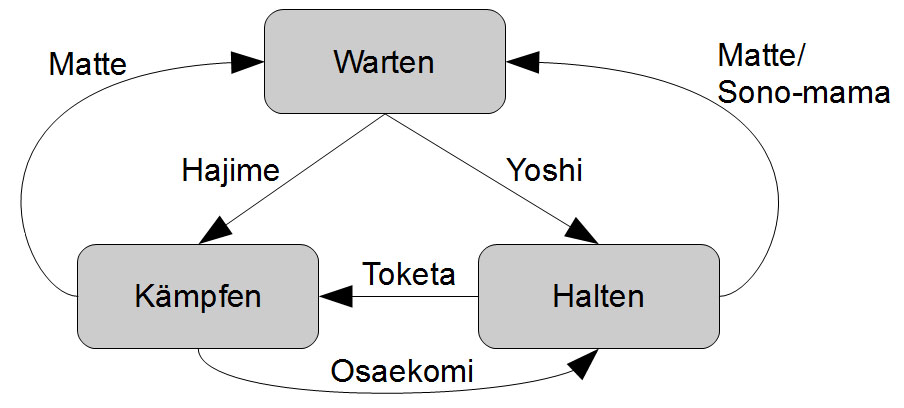
\includegraphics[width=0.80\textwidth]{Anleitung-img004.jpg}
\end{center}
F\"ur \textit{Sono-mama} muss man
w\"ahrend eines Haltegriffs Matte dr\"ucken. Die Haltegriffzeit wird
dann grau markiert (angehalten). Durch Dr\"ucken der jeweiligen
Haltegrifftaste kann der Haltegriff wieder aufgenommen werden
(\textit{Yoshi}).}

\clearpage
\chapter{Anhang}
\section[Computer f\"ur Zweischirmbetrieb vorbereiten]{Computer f\"ur Zweischirmbetrieb vorbereiten}
\label{bkm:AnhangDualView}\label{bkm:RefNumPara3241634018798}{\itshape
TODO...}

\end{document}
